\section{Method}

The code used for this project is based on the implementation code found in the following repository \cite{plvs2023hogdetection}.

Included in this paper's submission files are a README, python pip requirements file, evaluation figures, the model file, a training notebook, a validation notebook, and a sample notebook with a portion of the dataset for the reader to test the code.
To test the reader can run the sample notebook and see the model's predictions on the sample images.
If further testing is required, the README provides additional instructions for downloading the dataset and structuring the data.

% Preprocessing
\subsection{Preprocessing}

The dataset splits the images into training and validation data along with their respective annotations. 
The annotations are parsed so only the "person" annotation data is used.
The images are loaded and converted to greyscale.

The preparation of training data requires both positive and negative samples. 
Positive samples are extracted from the annotated person bounding boxes and assigned a label value of 1, while negative samples are derived from image regions outside these boxes and assigned a label value of 0. 

A sliding window approach generates feature extraction windows, using a fixed window size of (64, 128) pixels.
Once a sampling window is calculated, we then use the skimage \cite{vanderwalt2014scikit} HOG implementation to generate the feature data for that window.
The process is repeated for all the person bounding boxes in the image and for non-person regions. 
An example of the HOG extraction window is shown in Figure \ref{fig:hog_example}.

\begin{figure}[htbp]
  \centering
  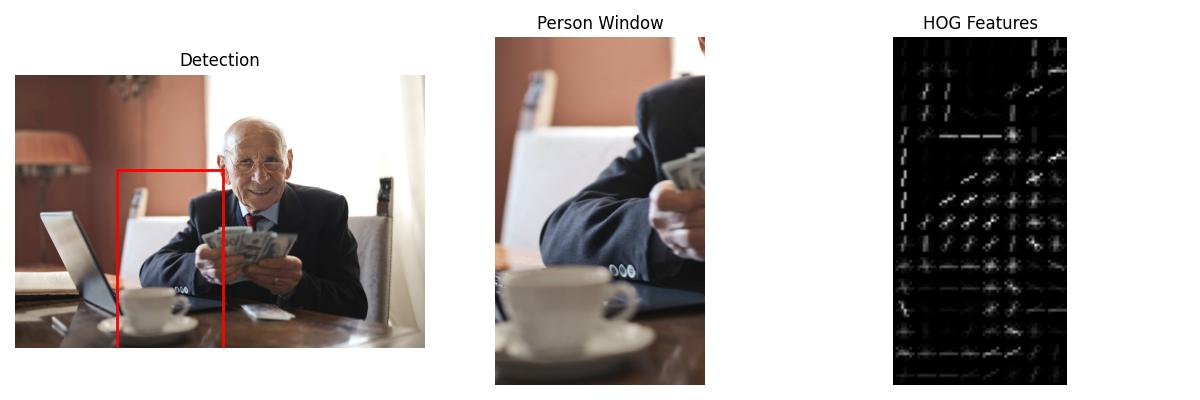
\includegraphics[width=0.9\linewidth,height=0.9\textheight,keepaspectratio]{hog}
  \caption{An example of the HOG feature extraction window during the evaluation process.}
  \label{fig:hog_example}
\end{figure}

An issue encountered by doing this is that without any limits on sample size we get a very large amount of negative samples for the dataset, greatly outnumbering the positive samples.
This could potentiality lead to overfitting, but more practically this was causing the training notebook to crash as the more than 100 batch files were generated of a few GBs of size. 

Initially a Linear Support Vector Classification (SVC)  was implemented for this training, but when the data batches were passed to the model for fitting, the memory usage exceeded the capabilities of the model code. 
At that point, I investigate alternative optimizer approaches and found \cite{sascha2017svm}, which suggested a SGD optimizer instead of the linear SVC due to the large amount of data.
In addition to the change of optimizer, a ratio of 5 negative to every positive sample was added to the sample generation to limit the number of negative samples.

\subsection{Training}

For training, an sklearn \cite{scikit-learn} pipeline is created using stochastic gradient descent (SGD) learning method and fit with a linear SVM. 

As described in the preprocessing section, the large amount of samples resulted in a exceeding the memory capabilities in the original implementation.
Given the large amount of sample data available, the SGD optimizer method is chosen as recommended in the sklearn documentation \cite{scikit-learn-map}.

The default parameters are used for training including a tolerance of 0.001 and a max iteration of 1000.
During the model fitting step the max iterations were met, thus convergence was not achieved in our training. 
Since SGD is sensitive to the feature scaling, the model input scaling in included in the model pipeline using the StandardScaler from sklearn.

In total 6479 images were loaded as training data with the following output:
\begin{itemize}
    \item Total features: 64990
    \item Positive samples: 10920
    \item Negative samples: 54070
    \item Feature dimension: 3780
\end{itemize}